\documentclass{article}
\usepackage[T1]{fontenc} 
\usepackage[utf8]{inputenc}
\usepackage{geometry}
\geometry{a4paper, textwidth=5.8in, textheight=9in}
\usepackage[export]{adjustbox}
\usepackage[final]{pdfpages}
\usepackage{graphicx}
\usepackage{float}
\usepackage{subcaption}
\usepackage{tabularx}
\usepackage[numbers]{natbib}
\usepackage[colorlinks=true,linkcolor=blue,citecolor=red,urlcolor=blue]{hyperref}
\usepackage{doi}
\graphicspath{{./Figures/}} 

%% Helper macros
\newcommand{\inlinepath}[1]{`\path{#1}'}
\newcommand{\hwport}[1]{\texttt{\detokenize{#1}}}
\newcommand{\parameter}[1]{\textit{\detokenize{#1}}}
\newcommand{\command}[1]{\texttt{\detokenize{#1}}}

%% FAQ style
\newcounter{troublecnt}[subsection]
%\renewcommand*\thetroublecnt{\arabic{section}.\arabic{troublecnt}}
\renewcommand*\thetroublecnt{Issue \arabic{troublecnt}}
\makeatletter
\newcommand\trouble{\@ifstar\troublenotnumbered\troublenumbered}
\makeatother
\newcommand{\troublenumbered}[1]{%
    \refstepcounter{troublecnt}%
    %{\it \makebox[1cm][l]{\textbf{\thetroublecnt}} #1}
    \begin{samepage}%
        \begin{description}%
            \item[\textbf{\thetroublecnt}] {\it #1}%
        \end{description}%
    \end{samepage}\nopagebreak[4]%
}
\newcommand{\troublenotnumbered}[1]{%
    \refstepcounter{troublecnt}%
    {\it #1}%
}

\begin{document}

\title{ZUMA User's Manual}
\author{Alexander D. Brant, Tobias Wiersema, Arne Bockhorn,\\ Monica Keerthipati, and Nithin S. Sabu}
\date{30.05.2020}
\maketitle
\tableofcontents

%\clearpage
\section{Introduction}
This repository contains the ZUMA FPGA overlay architecture system that was introduced by 
\begin{NoHyper}\citeauthor{brantlemieux2012ZUMA} in \citeyear{brantlemieux2012ZUMA}\end{NoHyper}~\cite{brantlemieux2012ZUMA,brant2013MT} and later extended by Wiersema, Bockhorn and Platzner~\cite{wiersemaBP2014ZUMAReconOS,wiersemaBP2016ZUMAReconOS} and several students of Paderborn University.

\clearpage
\noindent The folders contain a number of components needed to use ZUMA, as well as examples and tests.
The directory structure is as follows:\\[1.5mm]
\renewcommand{\arraystretch}{1.4}%
\begin{tabularx}{\textwidth}{lX}
    \hline 
    doc/               &  Contains this documentation.  \\
    example/           &  Contains a ZUMA preferences file, sample Verilog and timing SDF files, and a script to compile.  \\
    external/          &  Required third party tools as GIT submodules. \\
    misc/              &  Contains a patch that is required to use (the very old) VPR6 with ZUMA. \\
    source/            &  Scripts to generate the ZUMA Verilog components and bitstreams. \\
    tests/             &  Included scripts used to test ZUMA components. \\
    tests/integration/ &  Python unit tests to automatically assert the correct installation and behavior of the ZUMA scripts. \\
    verilog/           &  Verilog files used for building a ZUMA system, included platform specific and simulation files. \\
    license.txt        &  The license under which ZUMA can be used. \\
    Makefile           &  Global Makefile to prepare a working tool flow for overlay generation. \\
    toolpaths.py       &  Global path setup to tie in the third party tools -- can be adapted if the provided tool submodules shall not be used. \\
    \hline \\
\end{tabularx}

\section{Installation}
ZUMA scripts are written in Python, and require a valid Python install to run.
The scripts are tested with Python 2.7. To just get started, just run
\begin{verbatim}
make
\end{verbatim}
This will fetch and build all required tools and run a unit test that asserts the correct behavior of the tool chain. If this finishes with an \emph{OK}, then your ZUMA copy is ready to be used, and you can skip the rest of this section.
If you run into build errors, please refer to the failing tool's GitHub site for help.

\subsection{VTR flow}
The VTR\footnote{\url{https://verilogtorouting.org/}} tool set must also be installed in order to compile with ZUMA. 
ZUMA does not call the VTR flow directly, but tools thereof and requires files that are generated by them.

For convenience, a GIT submodule is located under \inlinepath{external/vtr} that points to a VTR version of the official VTR GitHub repository\footnote{\url{https://github.com/verilog-to-routing/vtr-verilog-to-routing}} that is known to work with this ZUMA version.
This included VTR version can be build by just issuing a standard \command{make} in ZUMA's top directory, or in the \inlinepath{external} subdirectory.

Should you want to use an existing VTR installation with theses scripts, you can adapt the variable VTR\_DIR that is used in scripts to find the VTR install. 
To change it globally, update the file \inlinepath{toolpaths.py} in the base directory to point to your installation location.

VPR versions prior to 7 (which are thus very old by now) do not automatically dump the routing resource graph and lack a command line switch to do so.
Since this file is needed by ZUMA, you need to activate the dumping of this file via a debug switch at compile time. 
For modern versions of VTR and VPR, you will not need to perform the following steps and can skip to the next section.

For VPR 6 a patch file is located in the directory \inlinepath{$VTR_DIR/vpr/SRC/route/}, which can be applied to the file \inlinepath{rr_graph.c} 
, by calling:
\begin{verbatim}
cat (ZUMA dir)/misc/patch.txt (VTR dir)/vpr/SRC/route/rr_graph.c > \
    (VTR dir)/vpr/SRC/route/rr_graph.c'
\end{verbatim}
The patch instructs VPR to always dump its routing graph to the file \inlinepath{rr_graph.echo}.
If using a different version, defining CREATE\_ECHO\_FILES in \inlinepath{rr_graph.c} will enable this functionality. 

\subsection{Yosys}
To enable an automatic verification of the functional equivalence between the generated overlay configuration and the original HDL specification, you additionally need Yosys\footnote{\url{http://www.clifford.at/yosys/}}.

For convenience, a GIT submodule is located under \inlinepath{external/yosys} that points to a Yosys version of the official Yosys GitHub repository\footnote{\url{https://github.com/YosysHQ/yosys}} that is known to work with this ZUMA version.
This included Yosys version can be build by just issuing a standard \command{make} in ZUMA's top directory, or in the \inlinepath{external} subdirectory.

Should you want to use an existing Yosys installation with theses scripts, you can adapt the variable yosysDir that is used in scripts to find the Yosys install. 
To change it globally, update the file \inlinepath{toolpaths.py} in the base directory to point to your installation location.


\section{Running the Tools}
\subsection{Running the Example}
Calling the Python script
\begin{verbatim}
compile.sh test.v    
\end{verbatim}
will automatically build the ZUMA system Verilog \inlinepath{ZUMA_custom_generated.v}, 
and a bitstream hex file \inlinepath{output.hex}, which can be used to synthesize and configure a ZUMA system. 
By passing other circuit files, modifying the example ZUMA configuration file \inlinepath{zuma_config.py}, or providing an alternative configuration file via the \emph{-{}-config} command line switch, custom architectures and bitstreams can be generated.

\subsection{ZUMA Tool Flow}
The detailed flow of tools to generate ZUMA overlays and configurations for them is depicted in Figure~\ref{fig:zumaflow}, adapted from~\cite{wiersemaBP2016ZUMAReconOS}.

It roughly works as follows: 
Starting with the ZUMA parameters in the \inlinepath{zuma_config.py} the \command{compile.sh} uses the templates stored in \inlinepath{source/templates/} to generate the architecture description of the overlay in VTR's XML format.
Leveraging this architecture description and the virtual circuit, e.g., \inlinepath{test.v}, the VTR flow (or more specifically ODIN II, ABC, and VPR) can deduce the complete routing resources of the overlay, which are saved into a file (custom format in VTR \(\leq\) 7 and XML in VTR 8), and can also synthesize, place and route the virtual circuit to the described architecture, resulting in descriptive files for the netlist, the placement and the routing.
The ZUMA scripts take all of these generated files and compute the correct configuration each programmable entity of the overlay, i.e., eLUTs and programmable interconnect points, and save the complete virtual configuration as ZUMA bitstream into the files \inlinepath{output.hex} and \inlinepath{output.hex.mif}.
While the former is the correct bitstream version as defined for ZUMA, the latter is an undecorated collection of only the configuration bits and nothing more, ready-to-use for inclusion by vendor tools as memory content.
\begin{figure}[htp]
    \centering
    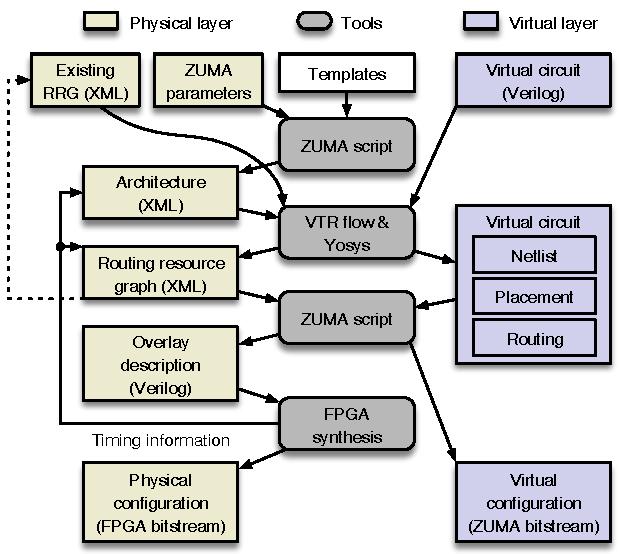
\includegraphics[width=0.7\textwidth]{Figures/zumaflow}%
    \caption{The tool flow to generate overlays and configurations.}
    \label{fig:zumaflow}
\end{figure}

For the physical side of things, the ZUMA scripts generate a description of the complete overlay fabric in Verilog, \inlinepath{ZUMA_custom_generated.v}, using LUTRAM instantiation macros to define all programmable entities.
This Verilog file can be included into a regular FPGA project to actually synthesize an overlay onto a physical device.
For more details of this inclusion, see Section~\ref{sec:include_ZUMA_in_project}.

\subsection{ZUMA Tool Flow Details}
The following sections highlight some flow details that happen automatically when running \command{compile.sh} and may thus be skipped by impatient readers.

\subsubsection{Generating the ZUMA Overlay Description}
To generate the Verilog architecture that can be synthesized to an FPGA, configuration files are generated for the VTR tools, 
which are then used to generate the global routing graph used in the ZUMA architecture.

\command{generate_buildfiles.py} generates the VPR architecture files and build scripts used during the compilation. 
It takes two arguments, a template input folder and an output folder. The script reads each template file in the input folder and substitutes specific keywords with the provided ZUMA parameters. This will generate the architecture file for VPR. 

VPR is then run (any BLIF file can be used), which outputs the routing resource graph, as well as the netlist, placement and routing files.

To generate the ZUMA system, \command{zuma_build.py} is called with the following parameters:
\begin{samepage}
\begin{verbatim}
python zuma_build.py
    -graph_file 'rr_graph.echo'
    -blif_file 'abc_out.blif'
    -place_file 'place.p'
    -route_file 'route.r'
    -net_file 'netlist.net'
    -bit_file 'output.hex'
    -blif_out_file 'zuma_out.blif'
    -verilog_file 'ZUMA_custom_generated.v'
\end{verbatim}
\end{samepage}
The filenames above are the default filenames used, and do not have to be specified if they are the same. 
The graph, BLIF, place, route and netlist files are all generated by earlier CAD steps, and are needed to generate the ZUMA 
configuration. 

The 'bit' file is the ZUMA bitstream in hex format, if this parameter is not specified the bitstream generation is not performed.
The Verilog file is the design file of the complete ZUMA system, that is used with other provided HDL files to run the ZUMA system.
The \inlinepath{blif_out} file is a BLIF file which corresponds to the ZUMA architecture configured to the loaded design, which can be verified 
to be equivalent to the input BLIF using ABC.

\subsubsection{Compiling to the ZUMA architecture}
Generating a bitstream for the ZUMA architecture is done in the same way as generating the architecture Verilog. Call \command{zuma_build.py}
 as above with the correct input files, and if a name for the output hex file is specified, a new bitstream will be generated.

\subsection{Bit to BLIF}
You can also reverse ZUMA's virtual synthesis and (re-)build a BLIF file from the generated bitstream. To this end, you can call the script 
\begin{verbatim}
>example/extract_logic_function.sh output.hex.mif output.blif HasClock HasReset
\end{verbatim}
where \inlinepath{output.hex.mif} is the bitstream you want to build your BLIF from,
\inlinepath{output.blif} the name of the BLIF file you want to create and \parameter{HasClock} and \parameter{HasReset} are two booleans [True/False] which indicate if the circuit uses a clock and\,/\,or a reset signal.
Those two signal properties cannot be read from the bitstream so you have to specify them.

Additionally the script requires the same \inlinepath{zuma_config.py} architecture parameter configuration that was used to build the \inlinepath{output.hex.mif} initially, because the architecture details can also not be read from the bitstream.

\subsection{Timing Analysis}
\emph{Note}: This section is currently only applicable to Xilinx devices.

\noindent First you have to generate a ZUMA overlay with a specific architecture 
described by your \inlinepath{zuma_config.py} configuration. 
For this generation the parameter \parameter{params.sdf} has to be turned off.
Then you can integrate the overlay into your design (cf.~Section~\ref{sec:include_ZUMA_in_project}) and extract the timing information from it by generating two SDF (standard delay format) files.

Assuming that your toplevel design has the name \emph{Top}, generate the first SDF file that contains the the routing delay information by issuing:
\begin{verbatim}
>netgen -s 1  -pcf Top.pcf -sdf_anno true -sdf_path "netgen/par" \
-ne -insert_glbl true -insert_pp_buffers false -w \
-dir netgen/par -ofmt verilog -sim Top.ncd Top_no_buffer.v
\end{verbatim}

Then generate the second SDF file that holds the flip flop delays (port delay + Tshcko):

\begin{verbatim}
>netgen -s 1  -pcf Top.pcf -sdf_anno true -sdf_path "netgen/par" \
-ne -insert_glbl true -insert_pp_buffers true -w \
-dir netgen/par -ofmt verilog -sim Top.ncd Top_with_buffer.v
\end{verbatim}

Copy the two generated files \inlinepath{Top_with_buffer.sdf} and \inlinepath{Top_no_buffer.sdf} to your \inlinepath{example/} directory and edit the parameters \parameter{params.sdfFileName} and \parameter{params.sdfFlipflopFileName} of your configuration.
Also you have to reactivate the \parameter{params.sdf} flag and edit the instance parameter.

After performing these steps, you can run the ZUMA \inlinepath{compile.sh} script with any virtual circuit to get its critical path. The path and resulting frequency \(f_{max}\) will be printed on the command line.


\section{Caveats and Restrictions}
A constraint for the virtual circuit file is that the head of the model must have the following signature:
\begin{verbatim}
verilog-module-name ([clock], reset, [input-name-1, input-name-2 , ... ])
\end{verbatim}
The clock and reset signal must have the given names and positions for the scripts to recognize their special behavior.
The reset is treated as the first input on the FPGA.
The declaration of a clock is optional.

The LUTRAMs used in the ZUMA architecture and contained in this repository are generated using Xilinx and Altera macros. To use a different LUTRAM or memory, instantiate it in the file \inlinepath{lut_custom.v}, and define a new platform (e.g., PLATFORM\_STRATIXIV) in the file \inlinepath{define.v} to select this LUTRAM.

Note that the Altera macros have not been maintained and that for the current ZUMA version thus only the Xilinx side is tested and guaranteed to work with current vendor tool flows.
Especially support for sequential virtual circuits has so far only been implemented for Xilinx projects. 

%\clearpage
\section{Including a ZUMA Overlay in a Project}
\label{sec:include_ZUMA_in_project}

Once the Verilog architecture is created, and a hex bitstream is generated, the ZUMA system can be compiled and used.
The generated Verilog file that describes the virtual fabric, along with the files in the \inlinepath{verilog/generic/} and \inlinepath{verilog/platform/(platform)/} directories should be included in a new Xilinx / Altera project, although getting it to work for Altera devices might require some (read: significant amount of) additional work.
We will describe the intent and general process here, for specific details on how to include it in a Xilinx Vivado project, please refer to Section~\ref{sec:include_ZUMA_in_Xilinx_project}.

The generated hex file should be placed in the project directory, and specified as the initial contents of the ZUMA configuration memory.
The top level file \inlinepath{ZUMA_TB_wrapper} includes a memory block which references the hex file \inlinepath{output.hex} that should be generated by the ZUMA tools and included with the project.
Note that sequential circuits are so far only supported in Xilinx projects. 

If you change the configuration memory size, or the configuration width, you have to create an appropriate new memory using the vendor tools. 
Runtime configuration of the ZUMA overlay is performed by loading each block of memory in the hex file to the port \hwport{config_data}, along with its address to \hwport{config_addr}, and asserting the corresponding \hwport{config_en} port.
Configuration completes when all data are loaded. 

The ports \hwport{fpga_inputs} and \hwport{fpga_outputs} provide the interface between the physical and virtual FPGA logic.
As described in the original ZUMA paper~\cite{brantlemieux2012ZUMA} and Brant's master's thesis~\cite{brant2013MT}, the pins are located at the edges of the array, begin at the grid coordinate (0,1), and increase in the Y direction first.
The pins can be fixed to correspond to those of the input Verilog by specifying a pin location file when running VPR placement. 

If you want to use the timing analysis or want to build a BLIF from a hex file,
see the timing and bit to BLIF readme files.

\clearpage
\subsection{Including a ZUMA Overlay in a Xilinx Vivado Project}
\label{sec:include_ZUMA_in_Xilinx_project}
For the inclusion of a generated ZUMA overlay into a Xilinx Vivado project, we provide a more detailed explanation here along with screenshots.
When following these steps, you should be able to synthesize a working, configurable ZUMA overlay with your project.

\begin{enumerate}

    \item Create a new project in Vivado by including the source files in the following directories:
    \begin{itemize}
        \item \path{verilog/generic}
        \item \path{verilog/platforms/xilinx}
    \end{itemize}
    Do not copy the files into the project, as they will be common to all projects. %Refer figure \ref{fig:addfiles}.

    %\begin{figure}[H]
    %\centering
    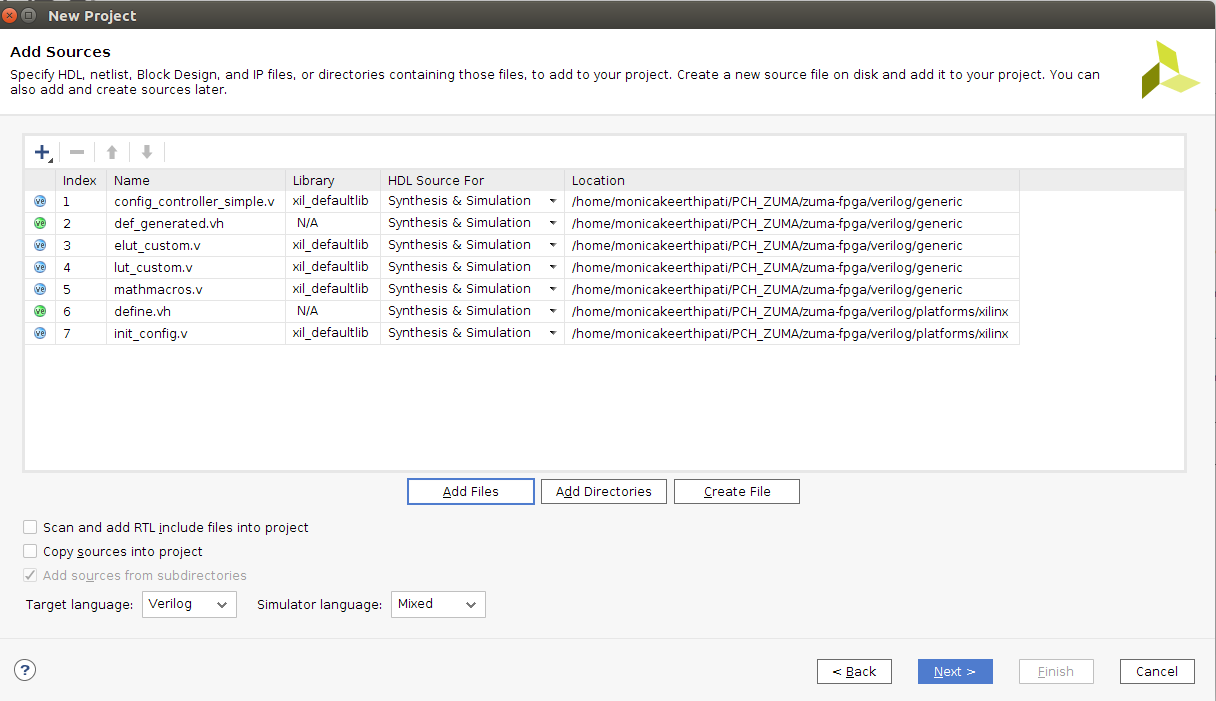
\includegraphics[width=.95\linewidth]{Figures/addfiles.png}
    %\label{fig:addfiles}
    %\end{figure}

    You might want to copy the file \inlinepath{verilog/generic/ZUMA_TB_wrapper.v} to the Vivado project, however, since this will be the top test bench for the project we are building here, so you might want to adapt this.

    %\begin{figure}[H]
    %\centering
    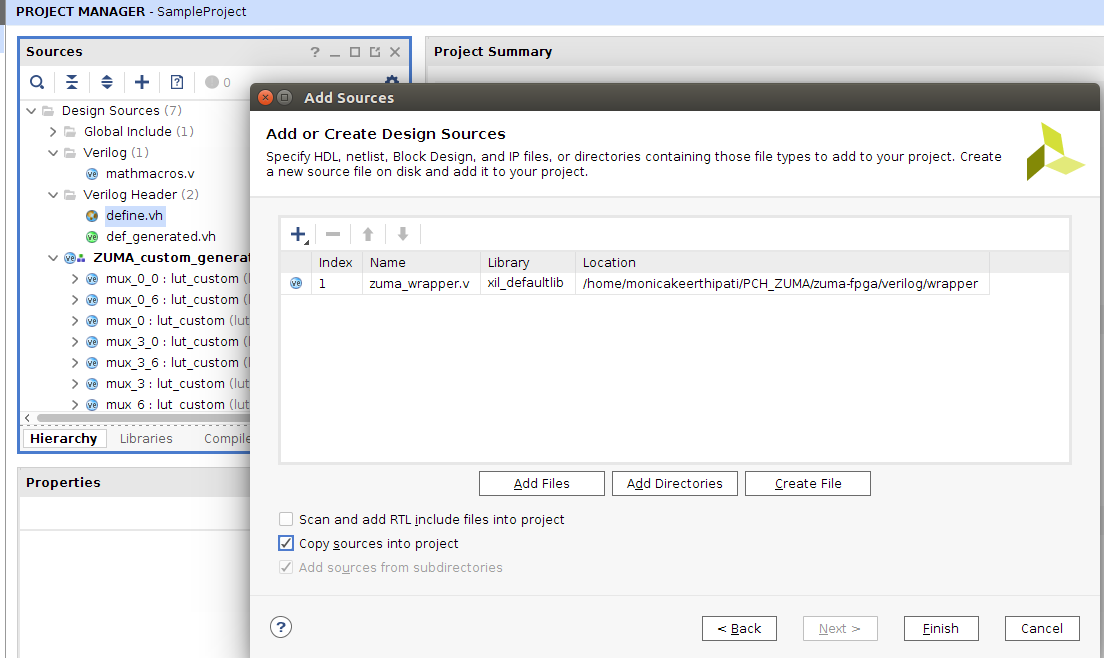
\includegraphics[width=0.95\linewidth]{Figures/vivado6.png}
    %\label{fig:vivado6}
    %\end{figure}

    \clearpage
    \item Click on \emph{Add sources} and add the following source files also to the project: %Refer figure \ref{fig:vivado5}.
    \begin{itemize}
        \item \path{example/ZUMA_custom_generated.v} -- overlay description
        \item \path{example/output.hex.mif} -- virtual configuration
        \item \path{example/def_generated.vh} -- generated header file
    \end{itemize}
    This time, you can choose whether or not to check \emph{Copy sources into project}. While these files change for each project, and thus could be copied, not copying them will force Vivado to read them from the ZUMA directory, so that when you regenerate them, they should be included in the new version.
    Should you, however, generate overlays for multiple projects in your ZUMA directory, it would be safer to copy them into the Vivado project.
    
    %\begin{figure}[H]
    %\centering
    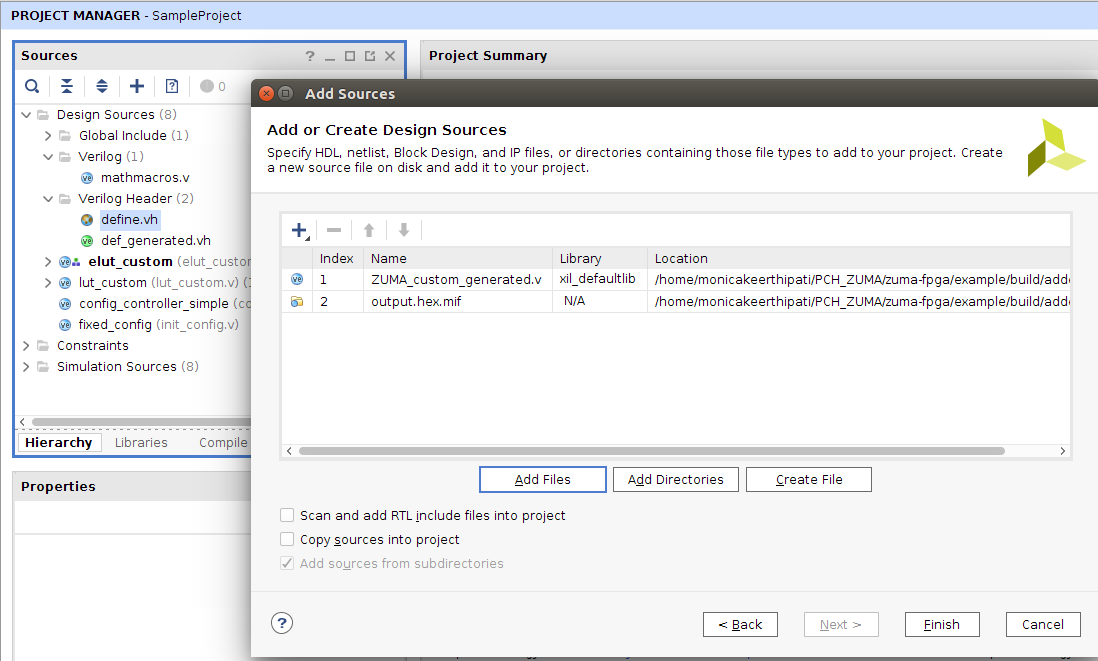
\includegraphics[width=0.95\linewidth]{Figures/vivado5.png}
    %\label{fig:vivado5}
    %\end{figure}
    
    %\clearpage
    \item Right click on \inlinepath{define.vh} and click \emph{Set Global Include} as shown. \\
    Do the same for \inlinepath{def_generated.vh}.%in figure \ref{fig:globalinclude}.

    %\begin{figure}[H]
    %\centering
    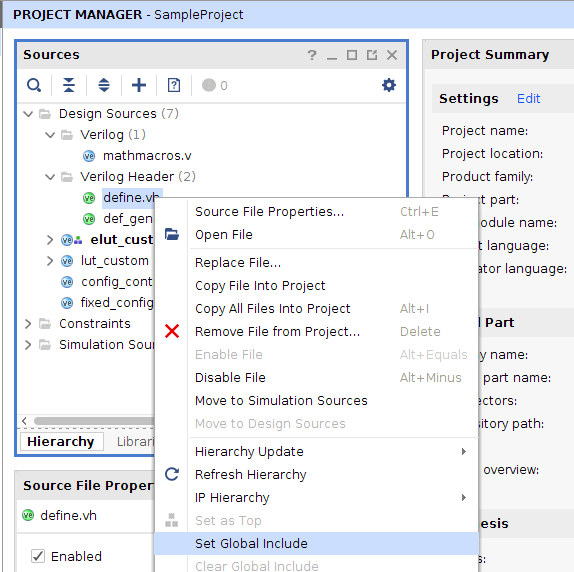
\includegraphics[width=0.5\linewidth]{Figures/globalinclude.png}
    %\label{fig:globalinclude}
    %\end{figure}

    \clearpage
    \item From the IP catalog, select the \emph{Distributed Memory Generator} core as shown. % in \ref{fig:vivado10}. 
    Change the component name to \hwport{lut_xilinx}. Set \emph{Data Width} to 1. Change \emph{Memory Type} to \emph{Simple Dual Port RAM} and click \emph{OK}. %Refer figure \ref{fig:vivado11} for this step.
    This will include the basic building block of ZUMA into the project -- the LUTRAMs -- which the overlay will instantiate a hundredfold.

    %\begin{figure}[H]
    %\centering
    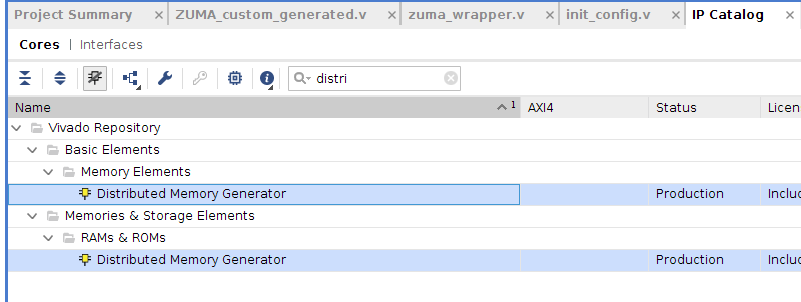
\includegraphics[width=0.7\linewidth]{Figures/vivado10.png}
    %\label{fig:vivado10}
    %\end{figure}

    %\begin{figure}[H]
    %\centering
    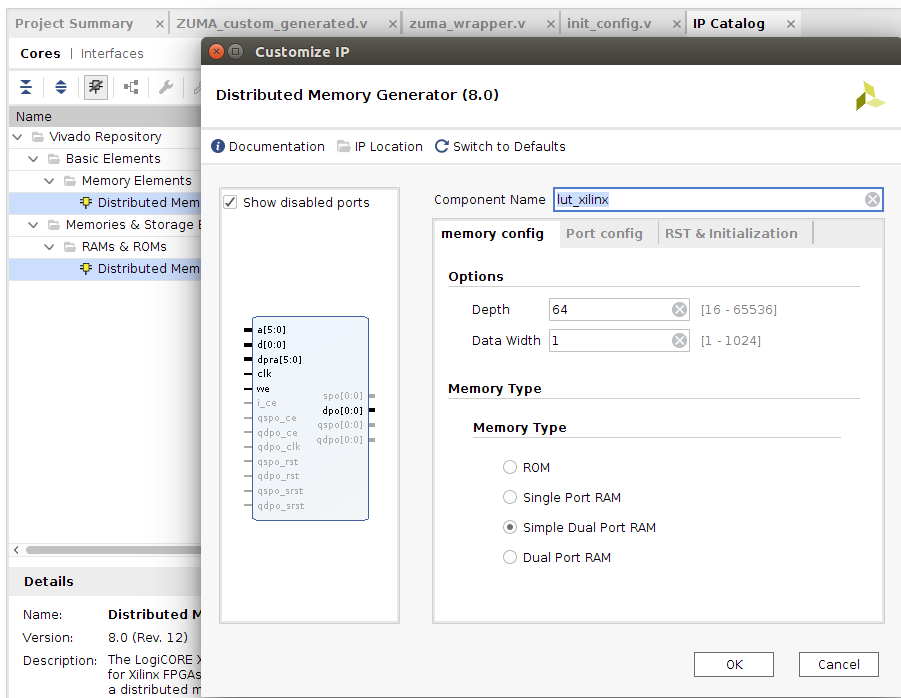
\includegraphics[width=0.7\linewidth]{Figures/vivado11.png}
    %\label{fig:vivado11}
    %\end{figure}
    
    \clearpage
    \item In the \emph{Generate Output Products} window that appears, set Synthesis Options to \emph{Out of context per IP} and click \emph{Generate}. %Refer figure \ref{fig:vivado12}.

    %\begin{figure}[H]
    %\centering
    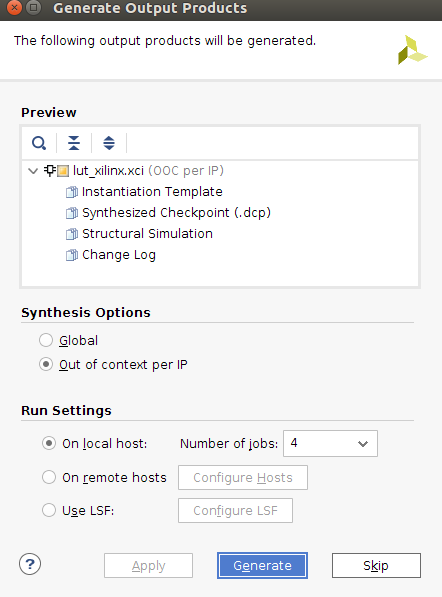
\includegraphics[width=0.5\linewidth]{Figures/vivado12.png}
    %\label{fig:vivado12}
    %\end{figure}
   
    \item Since the implementation of virtual sequential circuits, ZUMA requires a special version of this building block for its eLUTs. Hence, add the \emph{Distributed Memory Generator} core a second time now, but this time with different settings. Change the component name to \hwport{elut_xilinx}. Set \emph{Data Width} again to 1, and change \emph{Memory Type} also to \emph{Simple Dual Port RAM}. Do NOT dismiss the dialog, but proceed to the next tab now.

    %\begin{figure}[H]
    %\centering
    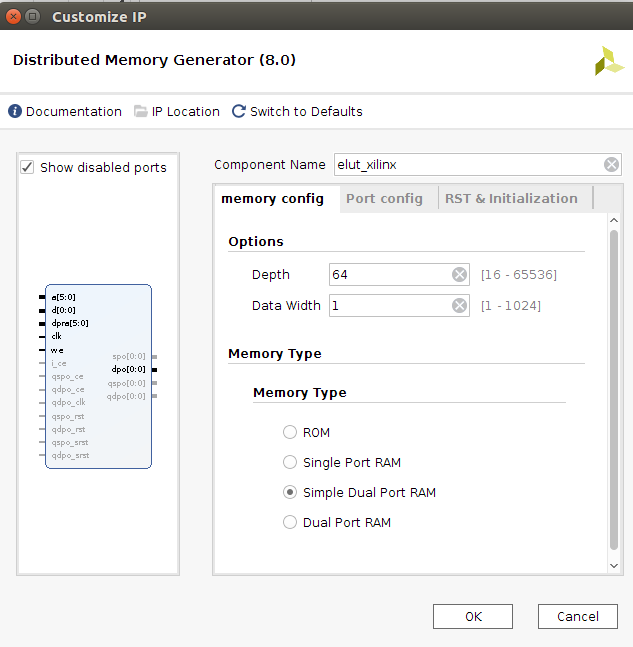
\includegraphics[width=0.7\linewidth]{Figures/vivado13.png}
    %\label{fig:vivado13}
    %\end{figure}

    In the \emph{Port config} tab, set \emph{Output Options} to \emph{Both}. Proceed to the final tab.

    %\begin{figure}[H]
    %\centering
    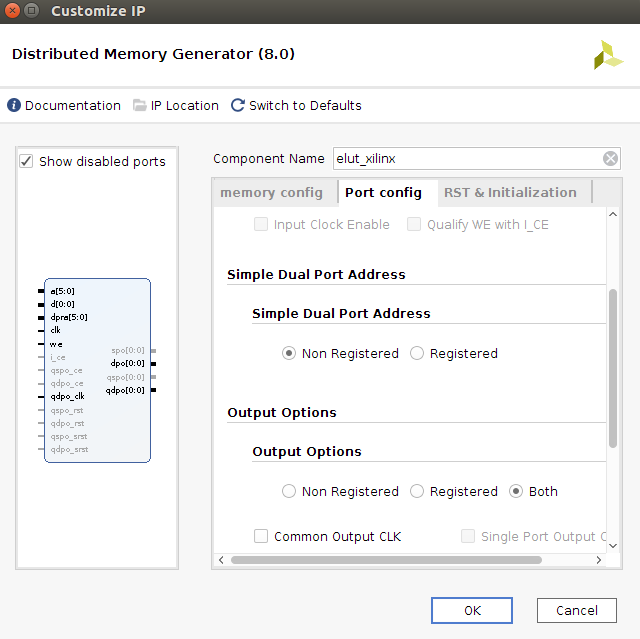
\includegraphics[width=0.7\linewidth]{Figures/vivado14.png}
    %\label{fig:vivado14}
    %\end{figure}

    In the \emph{RST and Initialization} tab, check \emph{Reset QSDPO} in \emph{Reset Options}.

    %\begin{figure}[H]
    %\centering
    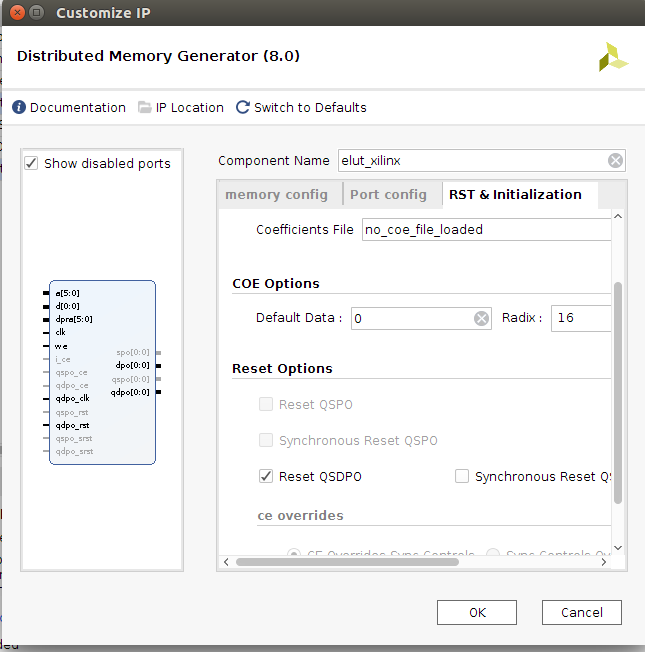
\includegraphics[width=0.7\linewidth]{Figures/vivado15.png}
    %\label{fig:vivado15}
    %\end{figure}

    Now you can finally click \emph{OK} and in the next window (\emph{Generate Output Products}) click \emph{Generate} again with \emph{Out of context per IP} settings. %The figures \ref{fig:vivado13}, \ref{fig:vivado14} and \ref{fig:vivado15} represent this step in a detailed manner.
    
    \clearpage
    \item Modify the \inlinepath{ZUMA_TB_wrapper.v} file based on your needs. It will be a good idea to remove the inputs and outputs from external ports and expose only part of it to the interface, since all ZUMA IO pins are general purpose IO pins and can thus be configured to be either an input or an output by the virtual configuration.
    The provided \hwport{fpga_inputs} and \hwport{fpga_outputs} are thus exactly twice the number of actually available IO pins, and there will not be enough pins to map all the inputs and outputs should you attempt to fully use both arrays for one configuration.
    Also, make sure to tie the unused inputs to ground, as otherwise, simulation will break.
 
\end{enumerate}

\subsubsection{Troubleshooting}

\trouble{Synthesis of the complete design is nearly impossible, since Vivado finds thousands of combinational loops.}
This might happen when you have a project that is a Vivado block design containing several IP cores, where one of them acts as the wrapper and configuration controller for the ZUMA overlay, and your follow the guide in this section to instantiate the customized \emph{Distributed Memory Generator} IP within.
This will probably seem to work fine, but the synthesis of the complete design can be nearly impossible as Vivado complains about thousands of combinational loops, crashing after running out of memory. This will then happen with the block design set to global synthesis, as well as with out-of-context synthesis. 

As it turns out, it is necessary to run out-of-context synthesis for each LUTRAM module. This way they are considered black boxes during final synthesis and timing loops are not reported. Unfortunately, Vivado has some serious limitations regarding nested block designs. The out-of-context synthesis products generated within the ZUMA wrapper IP are not recognized by Vivado, because nesting pre-synthesized IP cores in this manner is not supported. Some additional information can be found at \url{https://forums.xilinx.com/t5/Design-Entry/Limitations-of-the-Block-Designs/td-p/553937}

This problem can be solved by instantiating the LUTRAM modules from an .edif netlist. These can be generated by customizing the \emph{Distributed Memory Generator} IP in a new Vivado project, generating the output products, opening the resulting .dcp file with Vivado, and using the \command{write_edif} tcl command. This way the LUTRAM can be instantiated by simply including this .edif as a source file. An HDL stub definition of the module is needed though, at least for Verilog. This can be generated using the \command{write_verilog -mode port} command.
Details of this solution can be found at \url{https://forums.xilinx.com/t5/Design-Entry/Adding-xilinx-IP-dcp-files-for-packaging-custom-IP-to-speed-up/td-p/603142} and\\ also at \url{https://www.xilinx.com/support/answers/54074.html}.


\addcontentsline{toc}{section}{References}
\bibliographystyle{plainnat}
\bibliography{ZUMA}

\end{document}
